\usetikzlibrary{decorations.markings}%
\usetikzlibrary{decorations}%
\usetikzlibrary{decorations}%
\definecolor{body}{RGB}{200, 205, 200}%
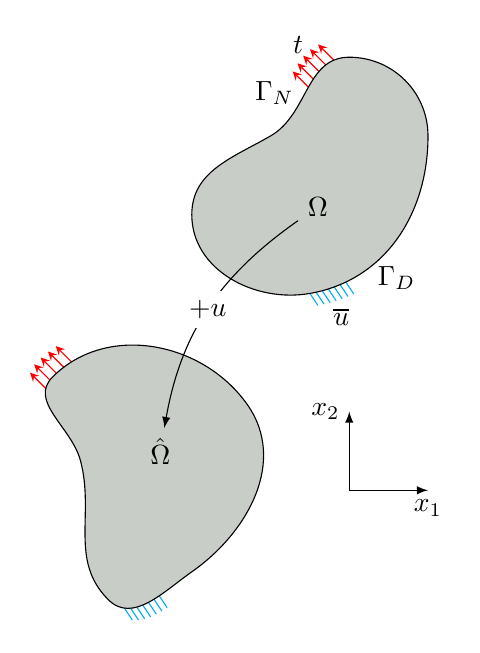
\begin{tikzpicture}
	% b.c.
	\draw[black, decorate, decoration = {
		markings,
		mark = between positions 0cm and 0.56cm step 0.8mm with {
			\draw[cyan] (0, 0) -- (0.1, -0.15);
		}
		pre = curveto,
		post = curveto,
		transform = {shift only},
	}]
	(1.5, 0.5) to[out = 10, in = -90]
	++(1.5, 2) to[out = 90, in = 0]
	++(-1, 1) to[out = 180, in = 30]
	++(-1, -1) to[out = -150, in = 90]
	++(-1, -1) to[out = -90, in = 190]
	cycle;

	\draw[black, decorate, decoration = {
		markings,
		mark = between positions 4.5cm and 5cm step 1.2mm with {
			\draw[red, -stealth] (0, 0) -- (-0.2, 0.2);
		}
		pre = curveto,
		post = curveto,
		transform = {shift only},
	}]
	(1.5, 0.5) to[out = 10, in = -90]
	++(1.5, 2) to[out = 90, in = 0]
	++(-1, 1) to[out = 180, in = 30]
	++(-1, -1) to[out = -150, in = 90]
	++(-1, -1) to[out = -90, in = 190]
	cycle;

	% org. problem
	\draw[black, fill = body]
	(1.5, 0.5) to[out = 10, in = -90]
	++(1.5, 2) to[out = 90, in = 0]
	++(-1, 1) to[out = 180, in = 30]
	++(-1, -1) to[out = -150, in = 90]
	++(-1, -1) to[out = -90, in = 190]
	cycle;

	% shifted
	\begin{scope}[shift = {(0cm, 0.5cm)}, yscale = 1, rotate = -45]

		% b.c.
		\draw[black, decorate, decoration = {
			markings,
			mark = between positions 3cm and 3.56cm step 0.8mm with {
				\draw[cyan] (0, 0) -- (0.1, -0.15);
			}
			pre = curveto,
			post = curveto,
			transform = {shift only},
		}]
		(1.5, -0.5) to[out = -10, in = 80]
		++(1, -2) to[out = -100, in = 0]
		++(-0.5, -1) to[out = 180, in = -30]
		++(-1.5, 1) to[out = 150, in = -90]
		++(-1, 0.5) to[out = 90, in = -190] (1.5, -0.5);

		\draw[black, decorate, decoration = {
			markings,
			mark = between positions 6.6cm and 7.1cm step 1.2mm with {
				\draw[red, -stealth] (0, 0) -- (-0.2, 0.2);
			}
			pre = curveto,
			post = curveto,
			transform = {shift only},
		}]
		(1.5, -0.5) to[out = -10, in = 80]
		++(1, -2) to[out = -100, in = 0]
		++(-0.5, -1) to[out = 180, in = -30]
		++(-1.5, 1) to[out = 150, in = -90]
		++(-1, 0.5) to[out = 90, in = -190]
		(1.5, -0.5);

		\draw[black, fill = body]
		(1.5, -0.5) to[out = -10, in = 80]
		++(1, -2) to[out = -100, in = 0]
		++(-0.5, -1) to[out = 180, in = -30]
		++(-1.5, 1) to[out = 150, in = -90]
		++(-1, 0.5) to[out = 90, in = -190]
		cycle;

	\end{scope}

	\draw[black, -latex] (2, -2) -- node[below, pos = 1] {$x_1$} ++(1, 0);
	\draw[black, -latex] (2, -2) -- node[left, pos = 1] {$x_2$} ++(0, 1);

	% domains
	\node (omegaOrg) at (1.6, 1.6) {$\Omega$};
	\node (omegaDef) at (-0.4, -1.5) {$\hat{\Omega}$};

	\draw[black, -latex] (omegaOrg) to[out = -145, in = 80 ] node[fill = white] {$ + \boldsymbol{u}$} (omegaDef);

	% b.c.
	\node at (1.35, 3.65) {$\boldsymbol{t}$};
	\node at (1.05, 3.05) {$\Gamma_N$};

	\node at (1.9, 0.2) {$\overline{\boldsymbol{u}}$};
	\node at (2.6, 0.7) {$\Gamma_D$};

\end{tikzpicture}
